	
	The above analog signal routing subsystem must be controlled by the user.  Because this device is designed to simplify the user experience, the user interface should be intuitive to use; no or few instructions should be needed to operate it.  The user interface should clearly indicate the current state of the signal routing, and the method by which the user can change the routing should be likewise linked to the physical signal connections being made.  To avoid disrupting the user from their focus on audio, the interface should be primarily visual and tactile in nature, as opposed to auditory.  For these reasons, the indication and actuation elements should be meshed, taking the form of push buttons with an integrated light.

	As described in Table \ref{tab:routing_outputs} above, each of the two inputs can be connected to each of the two outputs.  This includes cases where both inputs are connected to one or both of the outputs.  In no scenario can an output be connected to no input, which means that the user will never experience any "dead spots" where no sound can be heard.

	Qualitative tests were used to determine the effectiveness of such an indicator light.  An 8" $\times$ 1/2" $\times$ 1/4" clear acrylic sheet was cut using a laser cutter.  One side of this sheet was engraved with the same laser cutter in a continuous pattern to provide a rough surface off which light can reflect and refract.  An LED was lit and place on one end of the sheet, facing the 1/2" $\times$ 1/4" rectangular side.  When the LED was held within 5mm or so of the face, the acrylic appeared to illuminate when viewing either of the 8" $\times$ 1/2" faces.  Though a white LED was originally planned, a blue color shows more contrast with the surrounding environment, so this is the color that will be used.  This rapid prototyping was conducted in a brightly lit machine shop, with lighting conditions similar to that expected in a guitar retail store, suggesting that this system will work in its intended environment.

	\begin{figure}
		\centering
		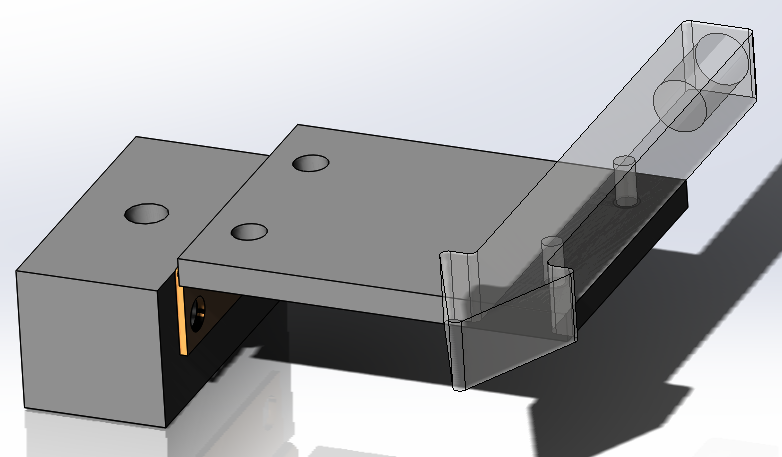
\includegraphics[width = 0.8\textwidth]{PR5Images/UIArrowCloseupCAD.png}
		\caption{Individual button setup for user interface showing the lever arm used to hold the indicator arrow light.}
		\label{fig:UIButtonCloseUp}
	\end{figure}

	Figure \ref{fig:UIButtonCloseUp} shows a single assembly for a light-button of this type, in this case illustrated without the button (the button and the lighting assembly are in separate CAD assemblies).  The clear arrow on top is a piece of 1/4" acrylic, with the bottom side raster textured on a laser cutter.  When light is injected into the acrylic from the side, it reflects off of this textured surface, which allows the light to be visible when looking down from the top view angle.  This arrow is mounted on a lever attached to a hinge, which is visible in a brass color.  This hinge pivots on a mounting block which is used to set the height of the arrow button.  A small pushbutton of the EVQ-22705R \cite{EVQ-22705Rdatasheet} variety is mounted underneath the lever directly below the center of the arrow.  When a user wants to select a routing connection, they would press down on the arrow.  This force produces a torque which allows the hinge to rotate down slightly, engaging the push button which pulls down an input on the microcontroller.

	Although this diagram illustrates a slot for a through hole LED to be inserted into the acrylic itself, rapid prototype testing indicated that the drill process for producing this slot causes too much texturing to the surface which interrupts the regular propagation of light the acrylic.  Therefore, small surface mount LEDs were used instead with no need for drilling.  

	\subsubsection{Button Layout}

	The exact layout of the buttons should be physically intuitive for the user to select the active inputs for each output.  The physically layout of the receivers is on a $3 \times 2$ grid.  The signal routing subsystems are used to connect the paired receivers on adjacent columns.  Figure \ref{fig:OverallUILayout} shows the overall layout of the receivers and the buttons.

	\begin{figure}
		\centering
		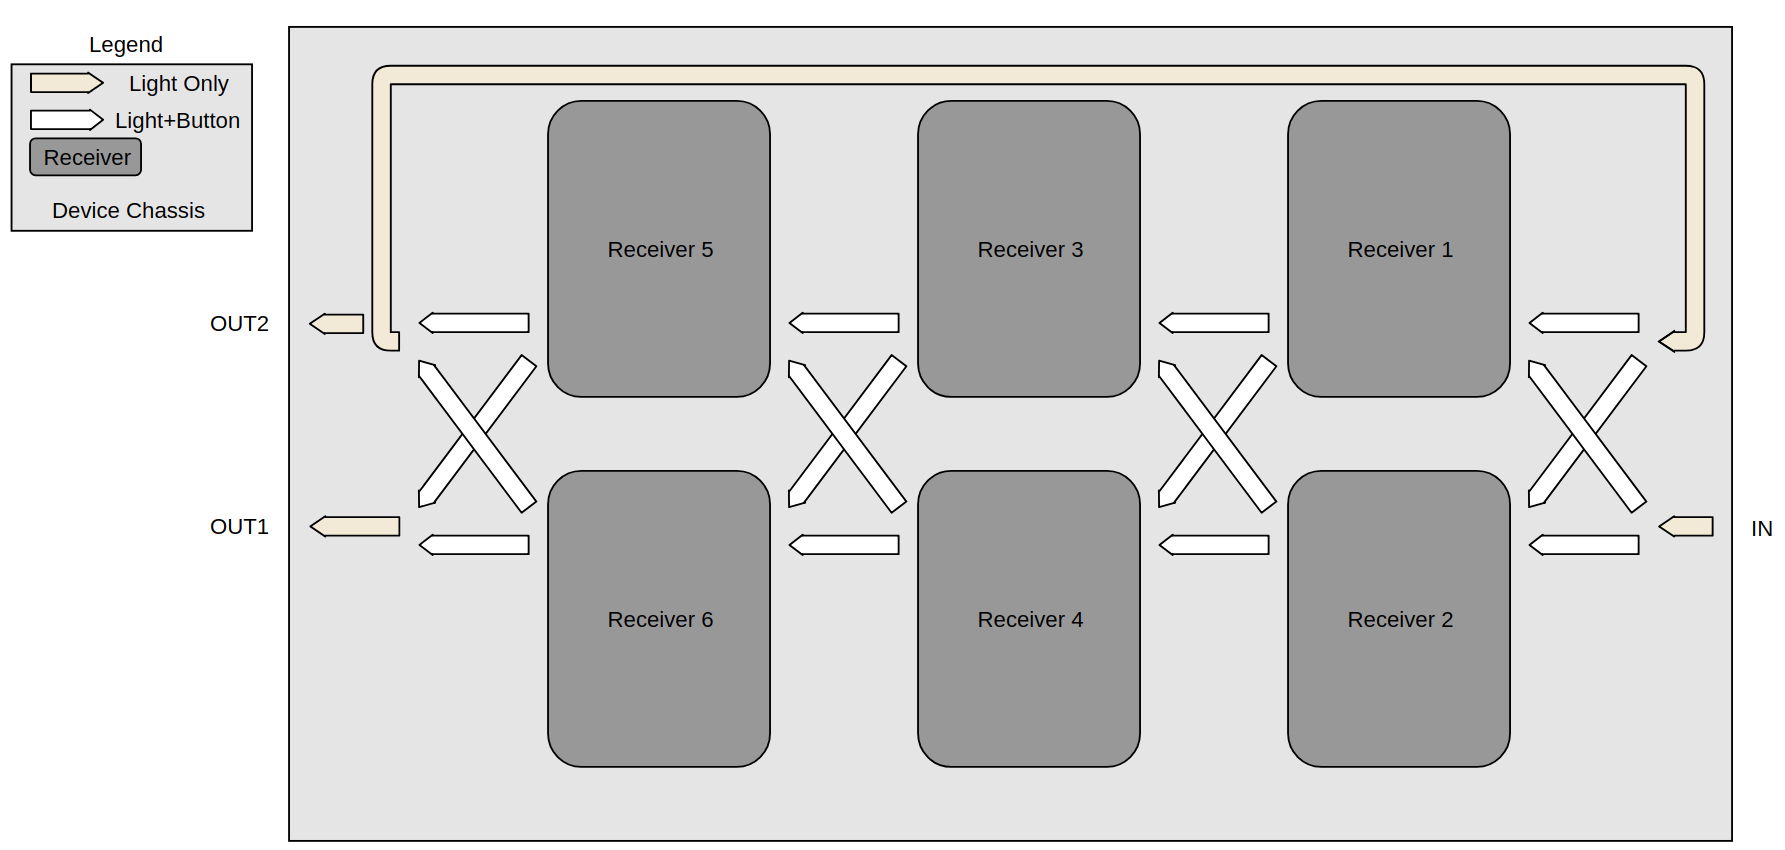
\includegraphics[width = \textwidth]{PR4Images/UIOverview.png}
		\caption{Overview of the user interface for understanding the physical layout of the overall unit.}
		\label{fig:OverallUILayout}
	\end{figure}

	To conform with guitar effects industry standards, the signal flow for the overall unit is from right to left.  Between each vertical pair of receivers (such as Receivers 1 and 2 in Figure \ref{fig:OverallUILayout} is a set of four integrated buttons and indicators, shown as white arrows.  Each set of these white arrows is connected to one module board and the board's routing subsystem.  Each button in the set is related to one particular signal routing direction.  For example, the arrow that points left from Receiver 2 to Receiver 4 indicates if the output of Receiver 2 is available on the input of Receiver 4.  In this example, that indicator would be lit if Receiver 4's input was either the output of Receiver 2 or the sum of the outputs of Receiver 1 and Receiver 2.  Each arrow shaped button toggles the state of both its LED and the relays associated with its connection.  In addition, there are a few lights, shown as tan arrows, that do not function as switches, and are lit depending on certain parameters.  For example, the indicators for IN, OUT1, and OUT2 are lit when a cable is plugged into the respective output to show that the connection has been correctly made.  In normal operation at a music store, the output will remain plugged in, so this functions as a de facto ON/OFF indicator.  The large indicator representing the feedback path turns on only when the feedback path is active: at least one of the two white arrows on the far right that point from the end of the feedback indicator into Receiver 1 and Receiver 2 are lit.

	In practice, the button-arrow assembly shown above is replicated several times, with different shaped pieces of acrylic to form the arrows.  These are mounted on a bracket which mechanically aligns the hinges from proper orientation.  This bracket has slots cut for the pushbuttons to be mounted with individual height adjustment so that the feel of the unit can be adjusted during fabrication.  Then the bracket and the pushbutton circuit boards are mounted on a larger base plate that connects the enclosure of the unit.  This is shown in Figure \ref{fig:UIASM}.

	\begin{figure}
		\centering
		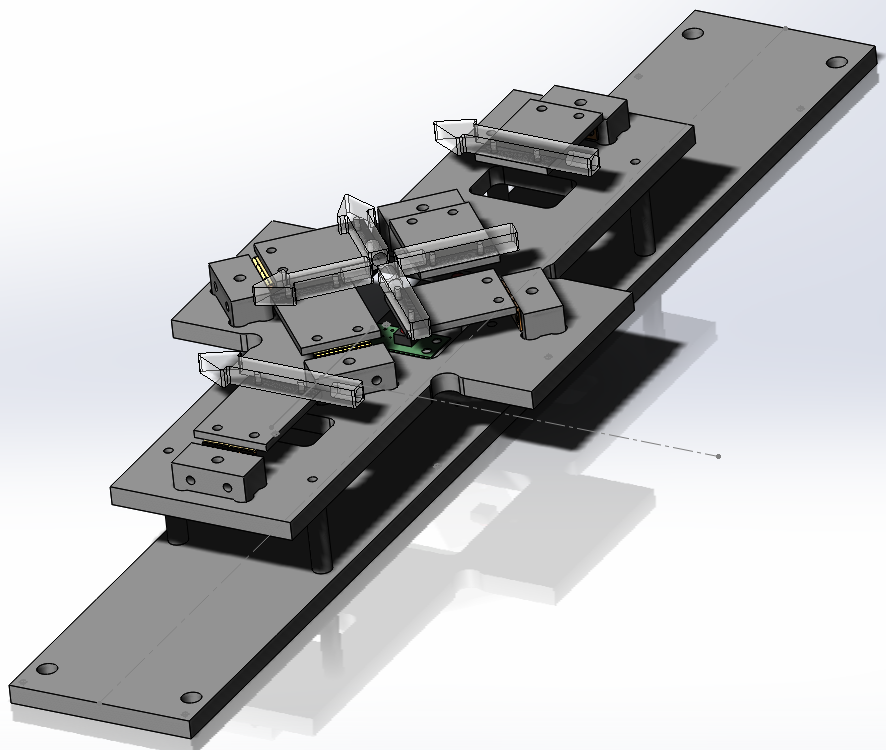
\includegraphics[width = 0.8\textwidth]{PR5Images/UIAsmCAD.png}
		\caption{User Interface subsystem assembly.  This shows the acrylic arrow lights, the circuit boards which hold the pushbuttons, and the assembly plate.}
		\label{fig:UIASM}
	\end{figure}

	\subsubsection{Control Finite State Machine}

	Each routing subsystem is a two input, two output mixer.  Each of the outputs can be the connected to either input or the sum of the inputs.  This means that these outputs can be controlled independently, so each set of white arrows can be split into two groups based on the output they control.  For instance, in Figure \ref{fig:UIarrowlabels}, buttons $a$ and $b$ control the top output while $c$ and $d$ control the bottom output.

	\begin{figure}
		\centering
		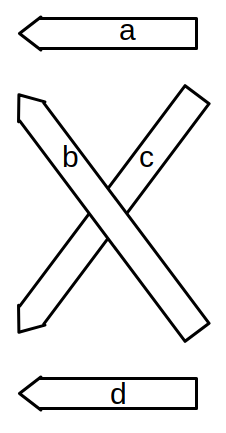
\includegraphics[width = 0.15\textwidth]{PR4Images/UIarrowlabels.png}
		\caption{Set of button-indicators.  These are associated with one module and are used to control the module's signal routing subsystem.  The letters are used for identification in this document.}
		\label{fig:UIarrowlabels}
	\end{figure}

	The switch logic and debouncing is computed on the microcontroller.  The finite state machine depicted in Figure \ref{fig:UIFSM} runs in two instantiations on the microcontroller to cover the $a$ and $b$ set of switches along with the $c$ and $d$ set.  This diagram illustrates only the machine associated with the $a$ and $b$ switches.  This is a Moore state machine where the output is determined by the current state.  The output/state is written in the boxes, and is described by STATE[1:0] where the bit 1 is the state of indicator $a$ and bit 0 is the state of indicator $b$.  The input vector is INPUT[1:0] where bits 1 and 0 represent whether switches $a$ and $b$ are asserted at any given time.

	\begin{figure}
		\centering
		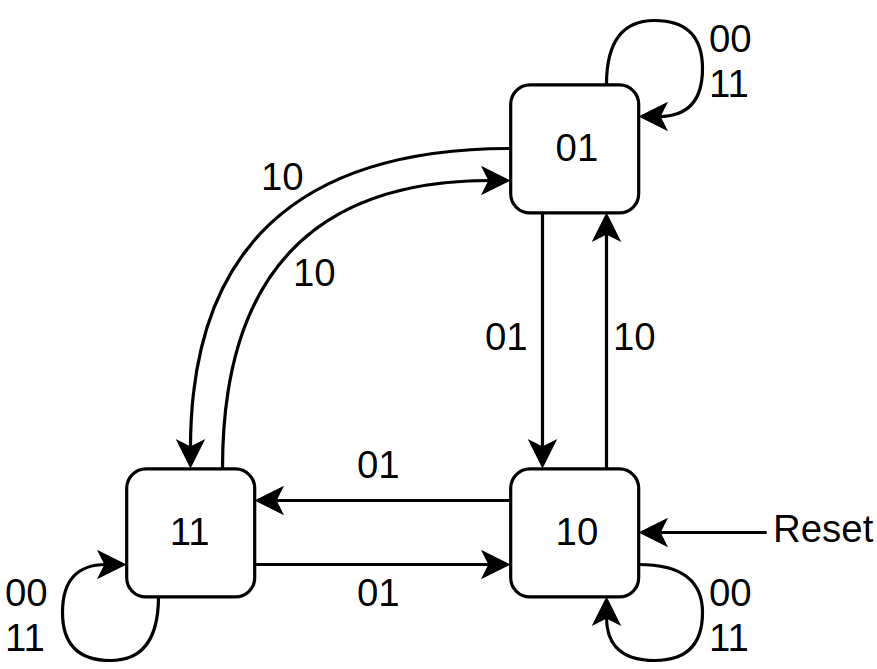
\includegraphics[width = 0.5\textwidth]{PR4Images/UIFSM.png}
		\caption{Finite State Machine describing the operation of the user interface for the signal routing.}
		\label{fig:UIFSM}
	\end{figure}

	As can be seen, the machine always starts in state $\mathtt{10}$, which means that the top input is connected to the top output in a "straight" line.  In terms of Figure \ref{fig:OverallUILayout}, this means that the unit will route the signal

	$$ \text{RECEIVER 1} \rightarrow \text{RECEIVER 3} \rightarrow \text{RECEIVER 5} $$

	This diagram does not indicate any information about the state of the relays in the actual signal routing subsystem.  This is because each FSM state, which is nominally tied to the LED state, also has a dedicated setting for those relays.  All of this information is summarized in a state transition table shown in Table \ref{tab:FSMtransitions}.  Note that state $\mathtt{00}$ should never be reached, as this would indicate that no output is currently selected.  If this state does mistakenly appear, it should transition to state $\mathtt{10}$, which is the default starting state.

	\begin{table}
	\begin{center}
	\begin{tabular}{ |c c|c c|c c|c c|}
	\hline
	\multicolumn{2}{|c|}{State/LED State} & \multicolumn{2}{|c|}{Relay Position} & \multicolumn{2}{|c|}{Input} & \multicolumn{2}{|c|}{Next State} \\
	\hline
	$a(d)$ & $b(c)$ & K1(K4) & K2(K3) & $a(d)$ & $b(c)$ & $a(d)$ & $b(c)$ \\
	\hline
	0 & 0 & 0 & 0 & X & X & 0 & 1 \\
	\hline
	\multirow{3}*{0} 	& \multirow{3}*{1} 	& \multirow{3}*{0} 	& \multirow{3}*{1} 	& 0 & 0 & 1 & 0 \\
						& 					&					&					& 0 & 1 & 1 & 0 \\
						& 					&					&					& 1 & 0 & 1 & 1 \\
						& 					&					&					& 1 & 1 & 0 & 1 \\
	\hline
	\multirow{3}*{1} 	& \multirow{3}*{0} 	& \multirow{3}*{0} 	& \multirow{3}*{0} 	& 0 & 0 & 1 & 0 \\
						& 					&					&					& 0 & 1 & 1 & 1 \\
						& 					&					&					& 1 & 0 & 0 & 1 \\
						& 					&					&					& 1 & 1 & 1 & 0 \\
	\hline
	\multirow{3}*{1} 	& \multirow{3}*{1} 	& \multirow{3}*{1} 	& \multirow{3}*{X} 	& 0 & 0 & 1 & 1 \\
						& 					&					&					& 0 & 1 & 1 & 0 \\
						& 					&					&					& 1 & 0 & 0 & 1 \\
						& 					&					&					& 1 & 1 & 1 & 1 \\
	\hline
	\end{tabular}
	\caption{Routing User Interface FSM transition table.  The table describes the states for the $a$ and $b$ switches, and with the $c$ and $d$ side in parenthesis.}
	\label{tab:FSMtransitions}
	\end{center}
	\end{table}

	The embedded software running on the ATMEGA3209 consists of two of these state machines, as well as two of the state machines that define the receiver operation.

	\subsubsection{Electrical Design}
	The electrical hardware design of the user interface is very simple.  The buttons are connected directly between pins on the ATMEGA3209 and ground, and pull down the inputs when they are activated.  The more interesting facet are the LED drivers.  They use a standard constant current LED driver circuit, controlled from the microcontroller.  Because the ATMEGA3209 has a limited maximum ground current, it cannot be used to drive the LEDs directly.  White LEDs are used for visual effect, and they are typically specified for a forward current of 20mA.  Figure \ref{fig:LEDdriver} shows the circuit.  The LED has a 3V forward voltage drop and should have a 20mA forward current.  This means that the collector voltage of the BJT may be no greater than 2V given the 5V supply.  Choosing an emitter voltage of 1.5V allows for a 500mV drop from the collector to the emitter to allow for variations in LED forward voltage.  R24 is used to set the current given this emitter voltage.  Because the base voltage should be one diode drop above the emitter, the resistive divider formed by R40 and R42 set the base voltage to be 1.9V.  A $\beta$ of 100 suggests that the base current will be 200$\mu$A.  This constant current source should keep the LEDs lit evenly.

	\begin{figure}
		\centering
		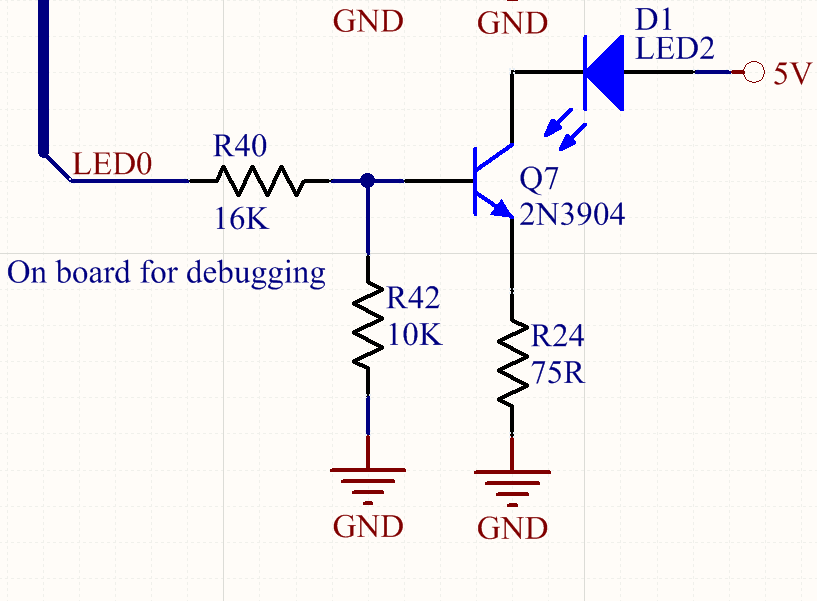
\includegraphics[width = 0.5\textwidth]{PR4Images/LEDconstcurrentdriver.PNG}
		\caption{Constant current source for LED.}
		\label{fig:LEDdriver}
	\end{figure}

